%\documentclass[convert]{standalone}
\documentclass[tikz,border=2pt]{standalone}
\usepackage{mhchem}
\usepackage{chemfig}
\usepackage{siunitx}
\begin{document}
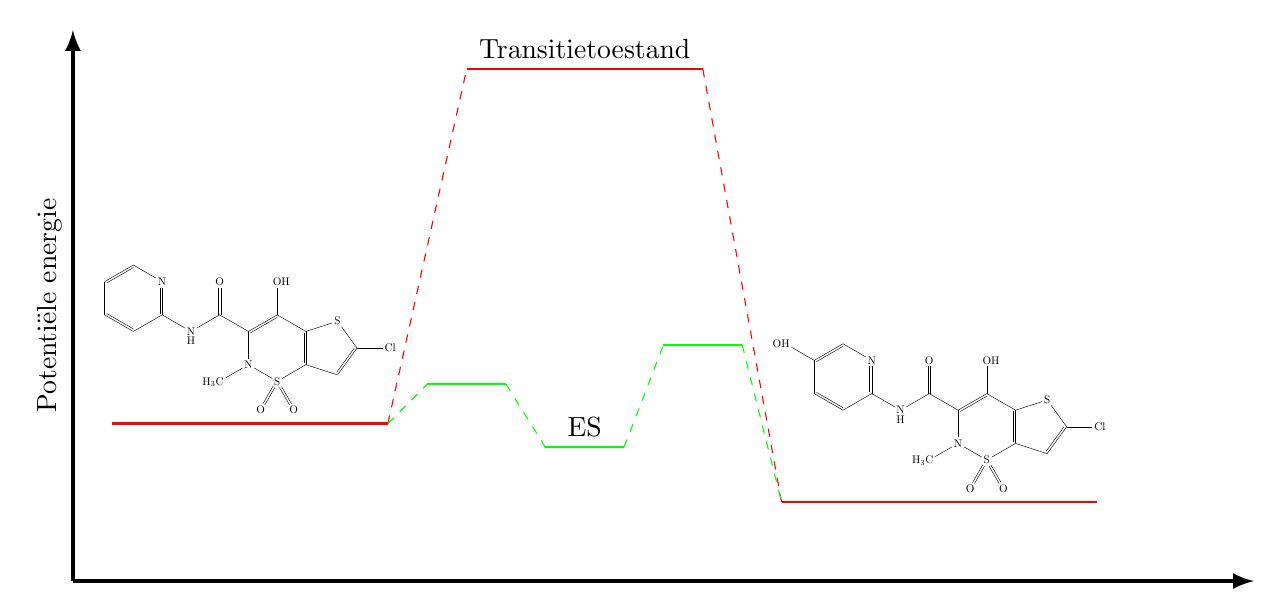
\begin{tikzpicture}
\draw[-latex,ultra thick] (0,0)--(15,0) ;
\draw[-latex,ultra thick] (0,0)--(0,7) node[midway,above,sloped]{Potenti\"ele energie};

\draw[-,thick,red] (0.5,2)--(4,2) node[midway,above,black]{\schemestart
	\scalebox{.4}{\chemfig{*6(=-(-[::-60]\chembelow{N}{H}-[::60](=[::+60]O)-*6(-N(-H_3C)-S(=[::-30]O)(=[::-90]O)-*5(-=(-Cl)-S--)=-(-OH)=))=N-=-)}}
	\schemestop};

\draw[-,red,dashed](4,2)--(5,6.5);
\draw[-,thick,red] (5,6.5)--(8,6.5)node[midway,above,black]{Transitietoestand};
\draw[-,dashed,red] (8,6.5)--(9,1);



\draw[-,green,dashed](4,2)--(4.5,2.5);
\draw[-,thick,green] (4.5,2.5)--(5.5,2.5);
\draw[-,dashed,green] (5.5,2.5)--(6,1.7);
\draw[-,thick,green] (6,1.7)--(7,1.7)node[midway,above,black]{ES};
\draw[-,dashed,green] (7,1.7)--(7.5,3);
\draw[-,thick,green] (7.5,3)--(8.5,3);
\draw[-,dashed,green] (8.5,3)--(9,1);


\draw[-,thick,red]  (9,1)--(13,1)node[midway,above,black]{\schemestart
	\scalebox{.4}{\chemfig{*6(=-(-[::-60]\chembelow{N}{H}-[::60](=[::+60]O)-*6(-N(-H_3C)-S(=[::-30]O)(=[::-90]O)-*5(-=(-Cl)-S--)=-(-OH)=))=N-=(-OH)-)}} 
	\schemestop};

%\draw[latex-latex] (4.2,3)--(4.2,5) node[midway,right,black]{$E_a = \SI{67.6}{\kilo \joule \per \mole}$}; ;


\end{tikzpicture}
\end{document}